% ANEXO------------------------------------------------------------------------

% \begin{anexosenv}
% \partanexos

% % Novo anexo-------------------------------------------------------------------
% \chapter{Coleta de Amostra do Solo}
% \label{chap:anexoColeta}

% A coleta da amostra de terra deve ser feita de tal forma que o material coletado represente o terreno onde será implantada uma cultura. Esse procedimento é realizado devido ao fato de que toda a recomendação de adubação para o talhão é calculada considerando essa amostra.

% \begin{figure}[H]
%     \centering
%     \caption{Coleta de Amostra do Solo}
%     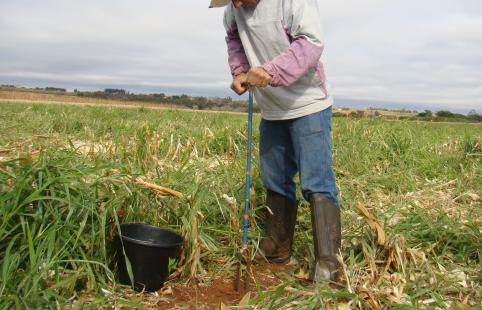
\includegraphics[width=13cm]{./dados/figuras/coleta_de_amostra_do_solo.jpg}
%     \label{fig:coletadeamostra}
%     \fonte{Sílvia Zoche Borges. Universo Agro.}
% \end{figure}

% \chapter{Laudo Técnico do Solo}
% \label{chap:laudodosolo}

% O laudo técnico do solo é um documento emitido por um laboratório especializado. Nele estão contidas informações como identificação do laboratório, propriedade, análise, nutrientes da terra e seus teores no solo.

% \begin{figure}[H]
%     \centering
%     \caption{Laudo Técnico do Solo}
%     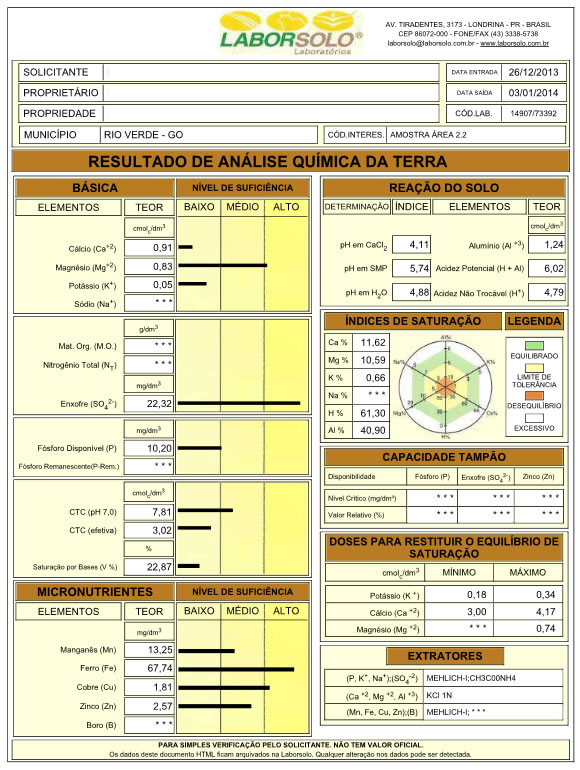
\includegraphics[width=13cm]{./dados/figuras/ex_analise_quimica.jpg}
%     \label{fig:laudotecnico}
%     \fonte{Roberto Antunes Fioretto. Doutores da Terra.}
% \end{figure}



% % Novo anexo-------------------------------------------------------------------
% \chapter{Quadro do Projeto no Trello}
% \label{chap:exemploQuadroTrello}

% Exemplo de organização das atividades do desenvolvimento da aplicação em um quadro no Trello. É possível observar a presença de listas e cartões com suas respectivas \textit{labels}, que definem a prioridade de desenvolvimento dos requisitos.

% \begin{figure}[H]
%     \centering
%     \caption{Exemplo de quadro de projeto no Trello}
%     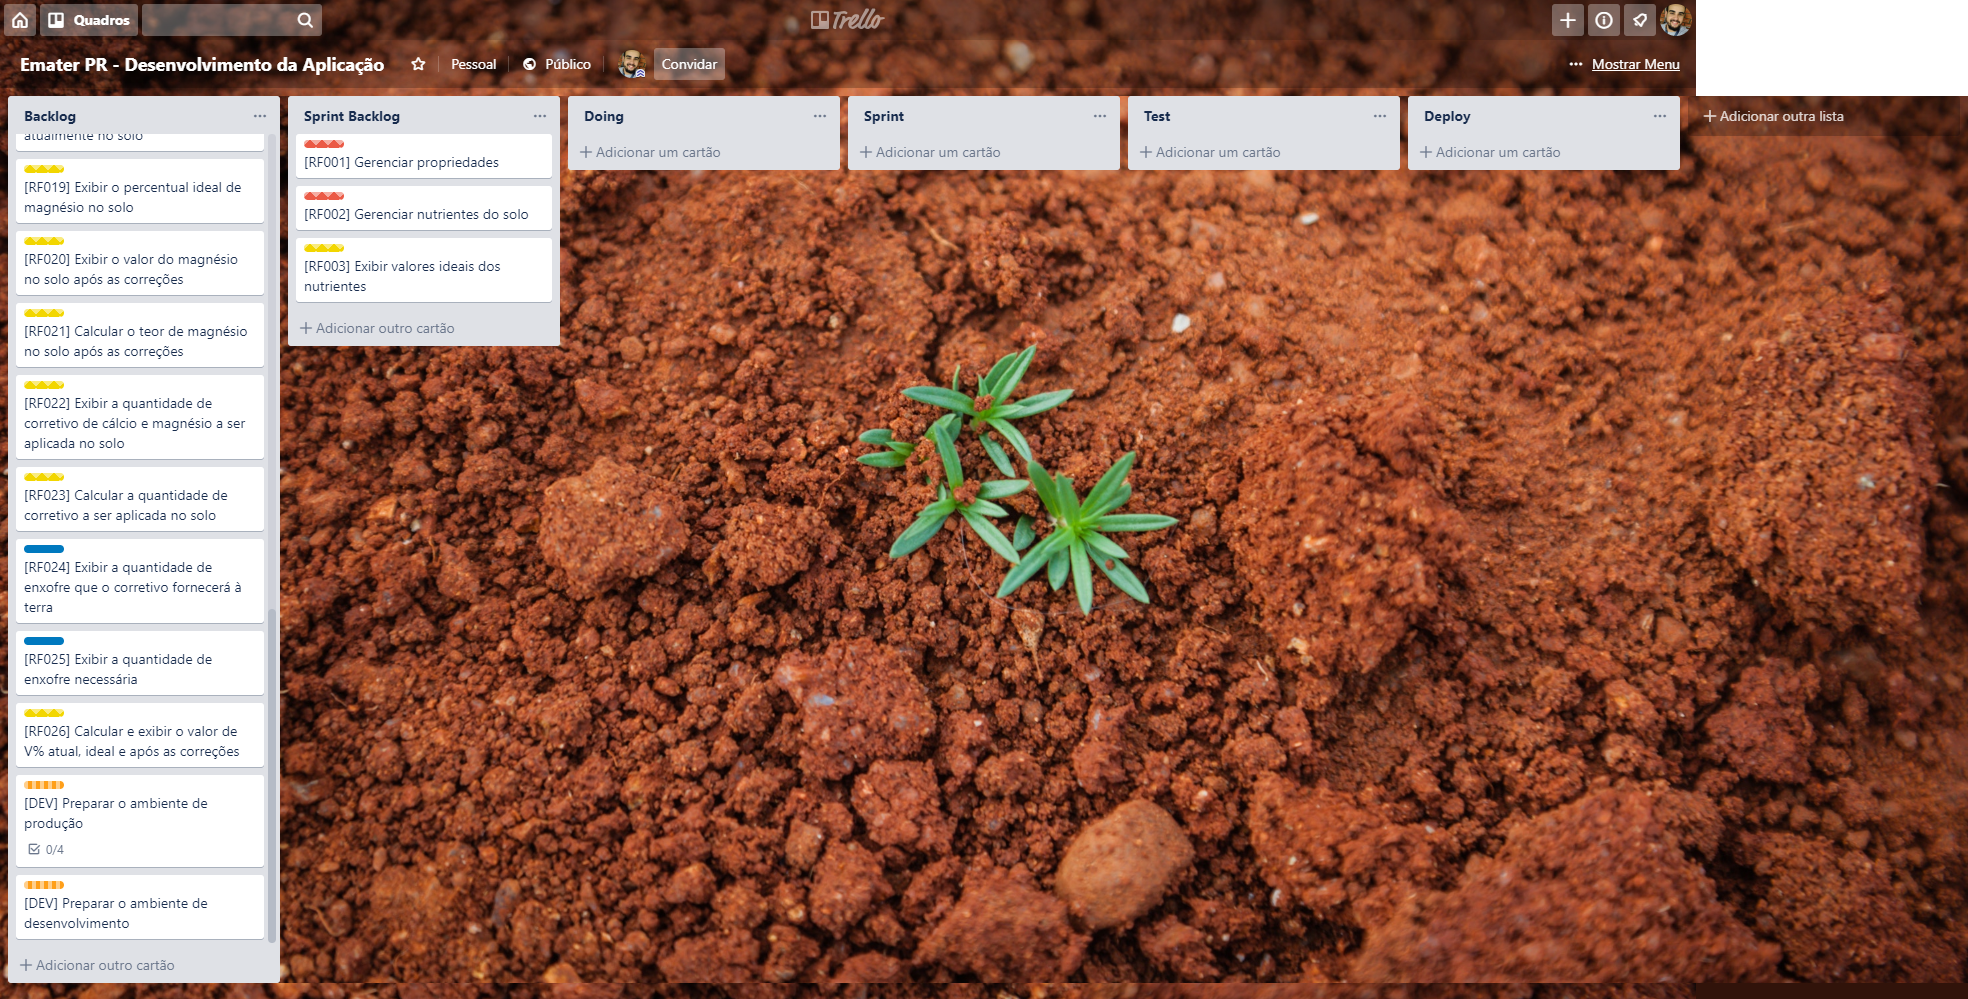
\includegraphics[width=13cm]{dados/figuras/quadro_trello.png}
%     \label{fig:exemploQuadroTrello}
%     \fonte{Autoria própria}
% \end{figure}


% \end{anexosenv}